% \iffalse
\let\negmedspace\undefined
\let\negthickspace\undefined
\documentclass[journal,12pt,twocolumn]{IEEEtran}
\usepackage{float}
\usepackage{circuitikz}
\usepackage{cite}
\usepackage{amsmath,amssymb,amsfonts,amsthm}
\usepackage{algorithmic}
\usepackage{graphicx}
\usepackage{textcomp}
\usepackage{xcolor}
\usepackage{txfonts}
\usepackage{listings}
\usepackage{amsmath}
\usepackage{enumitem}
\usepackage{mathtools}
\usepackage{gensymb}
\usepackage{comment}
\usepackage[breaklinks=true]{hyperref}
\usepackage{tkz-euclide} 
\usepackage{listings}
\usepackage{gvv}                                        
\def\inputGnumericTable{}                                 
\usepackage[latin1]{inputenc}                                
\usepackage{color}                                            
\usepackage{array}                                            
\usepackage{longtable}                                       
\usepackage{calc}  
\usepackage{caption}
\usepackage{multirow}                                         
\usepackage{hhline}                                           
\usepackage{ifthen}                                           
\usepackage{lscape}
\newtheorem{theorem}{Theorem}[section]
\newtheorem{problem}{Problem}
\newtheorem{proposition}{Proposition}[section]
\newtheorem{lemma}{Lemma}[section]
\newtheorem{corollary}[theorem]{Corollary}
\newtheorem{example}{Example}[section]
\newtheorem{definition}[problem]{Definition}
\newcommand{\BEQA}{\begin{eqnarray}}
\newcommand{\EEQA}{\end{eqnarray}}
\newcommand{\define}{\stackrel{\triangle}{=}}
\theoremstyle{remark}
\newtheorem{rem}{Remark}
\renewcommand\thesection{\arabic{section}}
\renewcommand\thesubsection{\thesection.\arabic{subsection}}
\renewcommand\thesubsubsection{\thesubsection.\arabic{subsubsection}}

\renewcommand\thesectiondis{\arabic{section}}
\renewcommand\thesubsectiondis{\thesectiondis.\arabic{subsection}}
\renewcommand\thesubsubsectiondis{\thesubsectiondis.\arabic{subsubsection}}
\lstset{
language=Python,
frame=single, 
breaklines=true,
columns=fullflexible
}
\numberwithin{equation}{subsection}
\renewcommand{\thesubsection}{\thesection.\arabic{subsection}}

\begin{document}

\bibliographystyle{IEEEtran}
\vspace{3cm}
\title{Audio Filtering}
\author{EE23BTECH11013 - Chedurtipati Avyaaz
}
\maketitle
\newpage
\bigskip
\renewcommand{\thefigure}{\arabic{figure}}
\renewcommand{\thetable}{\arabic{figure}}

\bibliographystyle{IEEEtran}

\tableofcontents

\begin{enumerate}[label=\thesection.\arabic*
,ref=\thesection.\theenumi]
\section{Digital Filter}
\label{input_sound}
\item Download the sound file from
\begin{lstlisting}
https://github.com/Avyaaz13/Audio-Filtering/blob/main/Audio%20Filtering/codes/Input_audio.wav
\end{lstlisting}
\item 
\label{Python code}
Below is the Python Code to perform the Audio Filtering:
\lstinputlisting{./codes/1.2_noise_red.py}\label{py:audio_filter}

\item 
\label{Visualization}

The audio file is analyzed using spectrogram using the online platform \label{prob:spectrogram}\href{https://academo.org/demos/spectrum-analyzer}{\url{https://academo.org/demos/spectrum-analyzer}}.

\begin{figure}[!ht]
    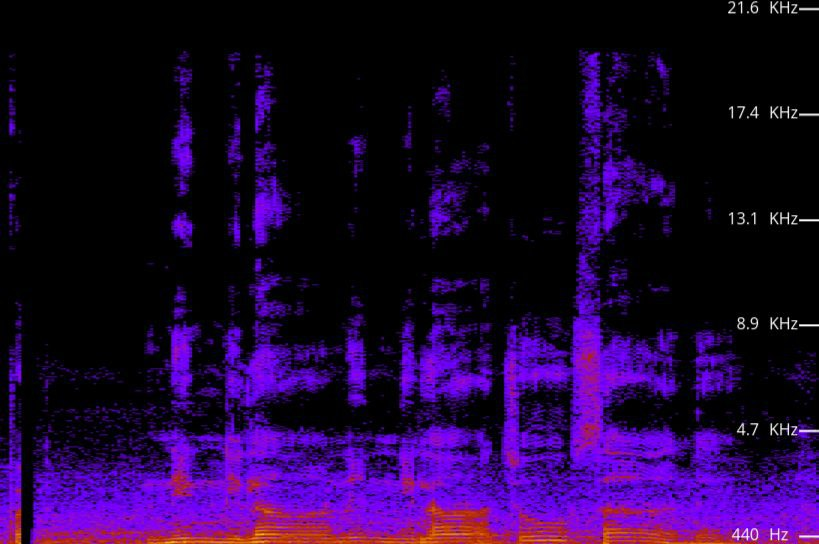
\includegraphics[width=\columnwidth]{figs/Input_audio_signal.jpg}
    \caption{Spectrogram of Input Audio}
    \label{fig:input_audio}
\end{figure}
\begin{figure}[!ht]
    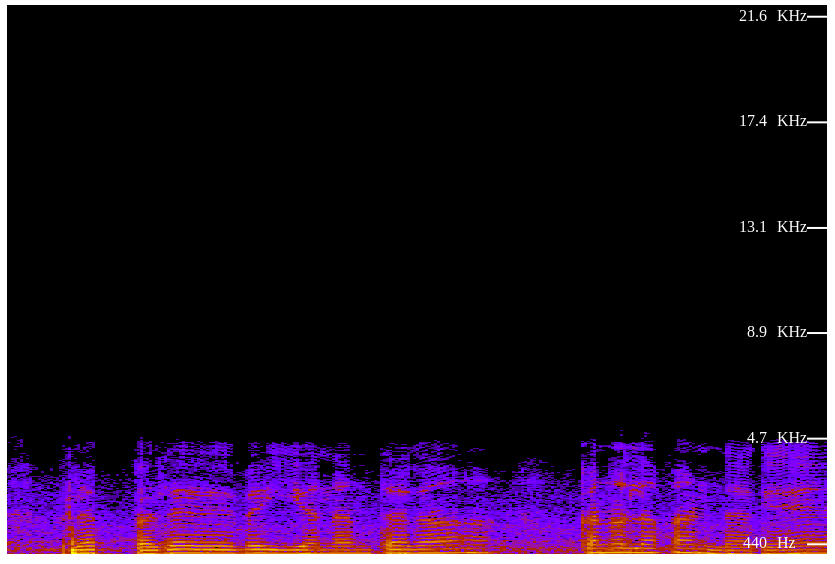
\includegraphics[width=\columnwidth]{figs/Filtered Output.png}
    \caption{Spectrogram of Filtered Input Audio}
    \label{fig:output_audio}
\end{figure}
\item
The output of the python script in Problem \ref{py:audio_filter} is the audio file ReducedNoise\_s181.wav. Play the file in the spectrogram in Problem \ref{prob:spectrogram}. What do you observe?
\\
\textbf{Solution:}The orange and yellow areas represent frequencies that have high intensities in the sound.
The key strokes as well as
background noise is subdued in the audio.
Also, the signal is blank for frequencies above
5.1 kHz.
\end{enumerate}

 \section{Difference Equation}
 \begin{enumerate}[label=\thesection.\arabic*,ref=\thesection.\theenumi]
\item Let
\begin{equation}
x(n) = \cbrak{\underset{\uparrow}{1},2,3,4,2,1} \label{q:2.1}
\end{equation}
Sketch $x(n)$. 
\item Let
\begin{multline}
y(n) + \frac{1}{2}y(n-1) = x(n) + x(n-2),
\\
y(n) = 0, n < 0 \label{q:2.2}
\end{multline}
Sketch $y(n)$.
Solve\\
\solution  The C code calculates $y\brak{n}$ and Python plots the graph.
\begin{lstlisting}
https://github.com/Avyaaz13/Audio-Filtering/blob/main/Audio%20Filtering/codes/2.2_xnyn.c
\end{lstlisting} 
Below are the plots of the $x(n)$ and $y(n)$:
\begin{lstlisting}
https://github.com/Avyaaz13/Audio-Filtering/blob/main/Audio%20Filtering/codes/2.2_xnyn.py
\end{lstlisting}

\begin{figure}[!ht]
	\centering
	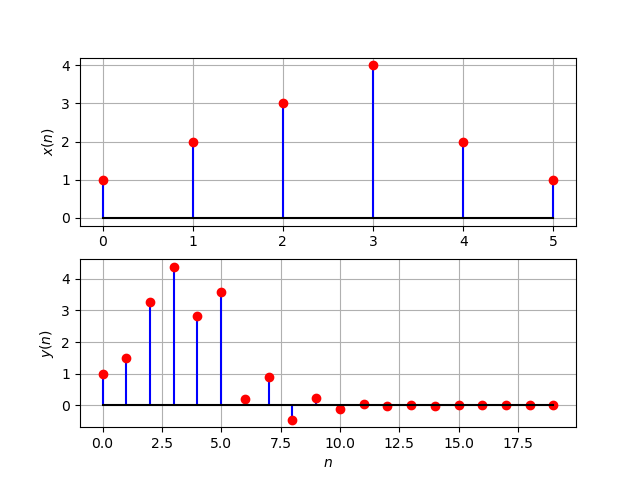
\includegraphics[width=\columnwidth]{figs/Plot_xnyn.png}
	\caption{Plot of $x(n)$ and $y(n)$}
	\label{fig:xnyn_graph}
\end{figure}
\end{enumerate}
\section{Z-Transform}

\begin{enumerate}[label=\thesection.\arabic*]
\item The $Z$-transform of $x(n)$ is defined as
%
\begin{equation}
\label{eq:z_trans}
X(z)={\mathcal {Z}}\{x(n)\}=\sum _{n=-\infty }^{\infty }x(n)z^{-n}
\end{equation}
%
Show that
\begin{equation}
\label{eq:shift1}
{\mathcal {Z}}\{x(n-1)\} = z^{-1}X(z)
\end{equation}
and find
\begin{equation}
	{\mathcal {Z}}\{x(n-k)\} 
\end{equation}
\solution From \eqref{eq:z_trans},
\begin{align}
{\mathcal {Z}}\{x(n-1)\} &=\sum _{n=-\infty }^{\infty }x(n-1)z^{-n}\\
n &\longrightarrow n+1\\ \nonumber
&=\sum _{n=-\infty }^{\infty }x(n)z^{-n-1} \\
&= z^{-1}\sum _{n=-\infty }^{\infty }x(n)z^{-n}\\
&= z^{-1}X(z)
\end{align}
resulting in \eqref{eq:shift1}. Similarly, it can be shown that
%
\begin{align}
{\mathcal {Z}}\{x(n-k)\} &=\sum _{n=-\infty }^{\infty }x(n-k)z^{-n}\\
n &\longrightarrow n+k \nonumber\\
&=\sum _{n=-\infty }^{\infty }x(n)z^{-n-k} \\
&= z^{-k}\sum _{n=-\infty }^{\infty }x(n)z^{-n}\\
&= z^{-k}X(z) \label{eq:z_trans_shift}
\end{align}
\item Find
%
\begin{equation}
H(z) = \frac{Y(z)}{X(z)}
\end{equation}
from  \eqref{q:2.2} assuming that the $Z$-transform is a linear operation.
\\
\solution  Using \eqref{eq:z_trans_shift} in \eqref{q:2.2},
\begin{align}
Y(z) + \frac{1}{2}z^{-1}Y(z) &= X(z)+z^{-2}X(z)
\\
\implies \frac{Y(z)}{X(z)} &= \frac{1 + z^{-2}}{1 + \frac{1}{2}z^{-1}}
\label{eq:freq_resp}
\end{align}
%
\item Find the Z transform of 
\begin{equation}
\delta(n)
=
\begin{cases}
1 & n = 0
\\
0 & \text{otherwise}
\end{cases}
\end{equation}
and show that the $Z$-transform of
\begin{equation}
\label{eq:unit_step}
u(n)
=
\begin{cases}
1 & n \ge 0
\\
0 & \text{otherwise}
\end{cases}
\end{equation}
is
\begin{equation}
U(z) = \frac{1}{1-z^{-1}}, \quad \abs{z} > 1
\end{equation}
\solution
\begin{align}
{\mathcal{Z}}\{\delta(n)\} &= \sum_{n=-\infty}^{\infty}\delta(n)z^{-n}\\
&= \delta(0)z^{-0}\\
&= 1
\end{align}
and from \eqref{eq:unit_step},
\begin{align}
U(z) &= \sum _{n= 0}^{\infty}z^{-n}
\\
&=\frac{1}{1-z^{-1}}, \quad \abs{z} > 1
\end{align}
%
\item Show that 
\begin{equation}
\label{eq:anun}
a^nu(n) \system{Z} \frac{1}{1-az^{-1}} \quad \abs{z} > \abs{a}
\end{equation}
\solution 
\begin{align}
	a^nu(n) &\system{Z} \sum_{n = 0}^{\infty}\brak{az^{-1}}^n \\
			&= \frac{1}{1-az^{-1}} \quad \abs{z} > \abs{a}
\end{align}
%
\item 
Let
\begin{equation}
	H\brak{e^{j \omega}} = H\brak{z = e^{j \omega}}.
\end{equation}
Plot $\abs{H\brak{e^{j \omega}}}$.  Comment.  $H(e^{j \omega})$ is
known as the {\em Discrete Time Fourier Transform} (DTFT) of $h(n)$.
\\
\solution Below is the code which plots the magnitude of Transfer Function:
\begin{lstlisting}
https://github.com/Avyaaz13/Audio-Filtering/blob/main/Audio%20Filtering/codes/3.5_H.py
\end{lstlisting}


The DTFT of a sequence \( x(n) \) is given by:
\[ H(e^{j\omega}) = \sum_{n=-\infty}^{\infty} x(n) e^{-j\omega n} \]

Now, consider \( H(e^{j(\omega + 2\pi)}) \):
\[ H(e^{j(\omega + 2\pi)}) = \sum_{n=-\infty}^{\infty} x(n) e^{-j(\omega + 2\pi) n} \]

Using Euler's formula,
\begin{align}
e^{-j(\omega + 2\pi) n} &= e^{-j\omega n} e^{-j2\pi n} = e^{-j\omega n} \\
\because  e^{-j2\pi n} &= 1\quad  \forall{n}
\end{align}
\begin{align}
  H(e^{j(\omega + 2\pi)}) = H(e^{j\omega}) 
\end{align}

Therefore, the fundamental period is $2\pi$ , which implies that DTFT of a signal is always periodic.

Substituting $z = e^{j \omega}$ in \eqref{eq:freq_resp}, we get
\begin{align}
	\left|H\brak{e^{j\omega}}\right| &= \left|\frac{1 + e^{-2j\omega}}{1 + \frac{1}{2}e^{-j\omega}}\right| \\
	 &= \sqrt{\frac{\brak{1 + \cos{2\omega}}^2 + \brak{\sin{2\omega}}^2}{\brak{1 + \frac{1}{2}\cos{\omega}}^2 + \brak{\frac{1}{2}\sin{\omega}}^2}}\\
	 &= \frac{4|\cos{\omega}|}{\sqrt{5 + 4\cos{\omega}}}
\end{align}
\begin{figure}[!ht]
\centering
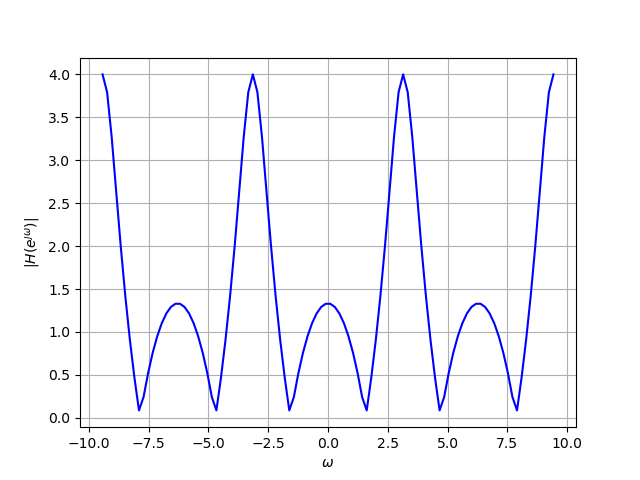
\includegraphics[width=\columnwidth]{figs/H(z).png}
\caption{$\abs{H\brak{e^{j\omega}}} \text{ vs } \omega$}
\label{fig:H(z)_3.5}
\end{figure}
\end{enumerate}

\section{Impulse Response}
\begin{enumerate}[label=\thesection.\arabic*]
\item \label{prob:impulse_resp}
Find an expression for $h(n)$ using $H(z)$, given that 
\begin{equation}
\label{eq:impulse_resp}
h(n) \system{Z} H(z)
\end{equation}
and there is a one to one relationship between $h(n)$ and $H(z)$. $h(n)$ is known as the {\em impulse response} of the
system defined by \eqref{q:2.2}.
\\
\solution From \eqref{eq:freq_resp},
\begin{align}
H(z) &= \frac{1}{1 + \frac{1}{2}z^{-1}} + \frac{ z^{-2}}{1 + \frac{1}{2}z^{-1}}
\\
\implies h(n) &= \brak{-\frac{1}{2}}^{n}u(n) + \brak{-\frac{1}{2}}^{n-2}u(n-2)
\end{align}
using \eqref{eq:anun} and \eqref{eq:z_trans_shift}.
\item Sketch $h(n)$. Is it bounded? Convergent? 
\\
\solution The following code plots $h\brak{n}$: 
\begin{lstlisting}
https://github.com/Avyaaz13/Audio-Filtering/blob/main/Audio%20Filtering/codes/4.2_h.py
\end{lstlisting}
\begin{figure}[!ht]
\centering
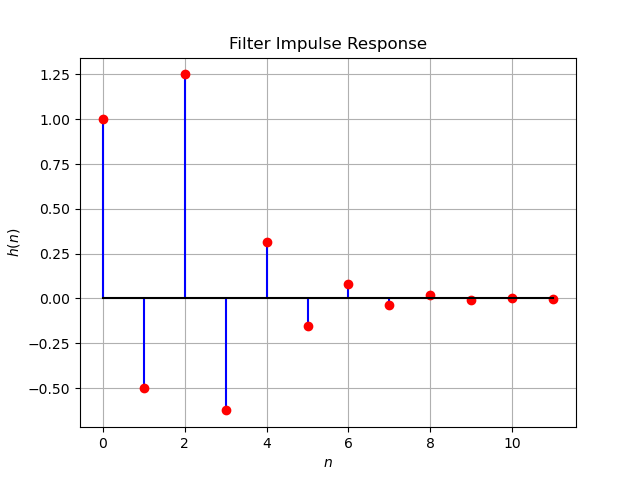
\includegraphics[width=\columnwidth]{figs/hn}
\caption{$h(n)$ \text{ vs } $n$}
\label{fig:hn}
\end{figure}
From graph, we can say that $h(n)$ is bounded.

To check for convergence we can use the ratio test:
\begin{align}
    \lim_{n \to \infty}\abs{\frac{h(n + 1)}{h(n)}} &= \abs{\frac{\brak{-\frac{1}{2}}^{n+1} + \brak{-\frac{1}{2}}^{n-1}}{\brak{-\frac{1}{2}}^{n} + \brak{-\frac{1}{2}}^{n-2}}}\\
    &= \frac{1}{2} < 1 \label{eq:5.5}
\end{align}
Hence, $h(n)$ is convergent.
\item The system with $h(n)$ is defined to be stable if
\begin{equation}
\sum_{n=-\infty}^{\infty}h(n) < \infty \label{eq:stb_condn}
\end{equation}
Is the system defined by \eqref{q:2.2} stable for the impulse response in \eqref{eq:impulse_resp}?\\
\solution Sum of infinite terms of a convergent series is finite. From \eqref{eq:5.5}, we proved that $h(n)$ was convergent therefore
\begin{equation}
\sum_{n=-\infty}^{\infty}h(n) < \infty
\end{equation}
Hence, the system with the impulse response $h(n)$ is a stable system.
\item 
Compute and sketch $h(n)$ using 
\begin{equation}
\label{eq:iir_filter_h}
h(n) + \frac{1}{2}h(n-1) = \delta(n) + \delta(n-2), 
\end{equation}

This is the definition of $h(n)$.
\\
\solution\\
{\em Definition of $h\brak{n}$}: The output of the system when $\delta\brak{n}$ is given as input.\\

Below code plots \figref{fig:hndef} which is same as the \figref{fig:hn}. 

\begin{lstlisting}
https://github.com/Avyaaz13/Audio-Filtering/blob/main/Audio%20Filtering/codes/4.4_hndef.py
\end{lstlisting}

\begin{figure}[!ht]
\centering
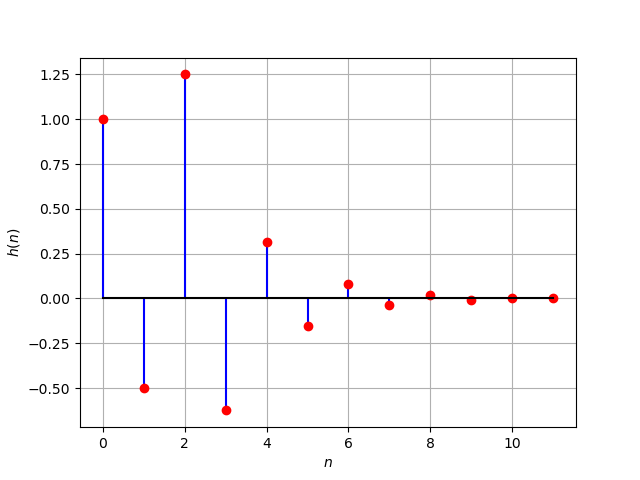
\includegraphics[width=\columnwidth]{figs/hndef}
\caption{$h(n)$ vs $n$ using definition}
\label{fig:hndef}
\end{figure}

\item Compute 
\begin{equation}
\label{eq:convolve_}
y(n) = x(n)*h(n) = \sum_{k=-\infty}^{\infty}x(k)h(n-k)
\end{equation}

Comment. The operation in \eqref{eq:convolve_} is known as
{\em convolution}.
%
\\
\solution Below code plots \figref{fig:ynconv_1} which is same as 
$y(n)$ in
\figref{fig:xnyn_graph}. 

\begin{lstlisting}
https://github.com/Avyaaz13/Audio-Filtering/blob/main/Audio%20Filtering/codes/4.5_ynconv.py
\end{lstlisting}
\begin{figure}[!ht]
\centering
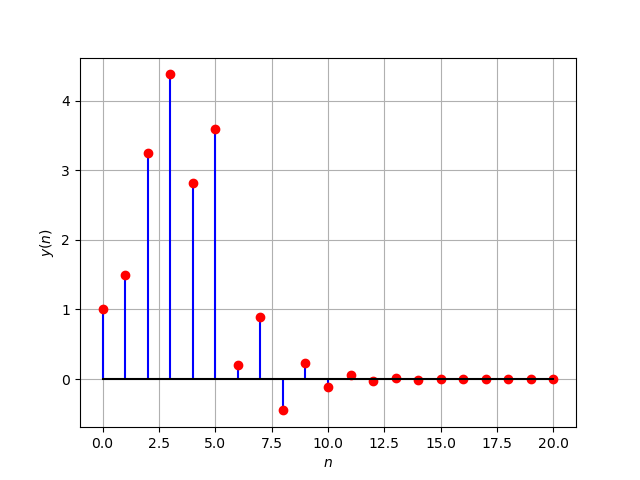
\includegraphics[width=\columnwidth]{figs/y_by_conv.png}
\caption{$y(n)$ from the definition of convolution}
\label{fig:ynconv_1}
\end{figure}

\item Show that
\begin{equation}
y(n) =  \sum_{k=-\infty}^{\infty}x(n-k)h(k)\label{conv}
\end{equation}
\solution
From, \eqref{eq:convolve_}
\begin{align}
y\brak{n} = \sum_{k=-\infty}^{\infty}x\brak{k}h\brak{n - k} 
\end{align}
Substitute $k \to n-k$:
\begin{align}
		  &= \sum_{n - k=-\infty}^{\infty}x\brak{n - k}h\brak{k} \\
		  &= \sum_{k=-\infty}^{\infty}x\brak{n - k}h\brak{k}
\end{align}
\end{enumerate}

\section{DFT and FFT}
\begin{enumerate}[label=\thesection.\arabic*]
\item
Compute
\begin{equation}
X(k) \define \sum _{n=0}^{N-1}x(n) e^{-\j2\pi kn/N}, \quad k = 0,1,\dots, N-1
\end{equation}
and $H(k)$ using $h(n)$.
\item Compute 
\begin{equation}
Y(k) = X(k)H(k)
\label{eq:fp}
\end{equation}
\item Compute
\begin{equation}
y\brak{n}={\frac {1}{N}}\sum _{k=0}^{N-1}Y\brak{k}\cdot e^{\j 2\pi kn/N},\quad n = 0,1,\dots, N-1
\label{eq:I-FT}
\end{equation}

\solution The above three questions are solved using the code below.
\begin{lstlisting}
https://github.com/Avyaaz13/Audio-Filtering/blob/main/Audio%20Filtering/codes/5.1_2_3.py
\end{lstlisting}
\begin{figure}[!ht]
\centering
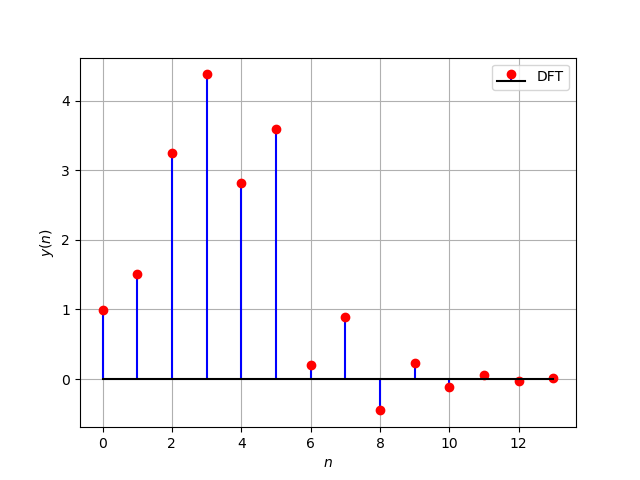
\includegraphics[width=\columnwidth]{figs/yn_DFT.png}
\caption{$y(n)$ obtained from DFT}
\end{figure}
\item Repeat the previous exercise by computing $X(k), H(k)$ and $y(n)$ through FFT and IFFT.
\solution The solution of this question can be found in the code below.
\begin{lstlisting}
https://github.com/Avyaaz13/Audio-Filtering/blob/main/Audio%20Filtering/codes/5.4_FFT.py 
\end{lstlisting}
\begin{figure}[!ht]
\centering
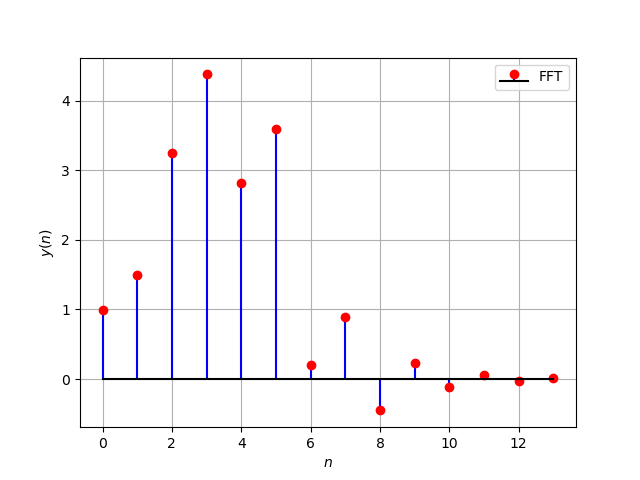
\includegraphics[width=\columnwidth]{figs/yn_FFT.png}
\caption{$y(n)$ obtained using IFFT}
\label{fig:yn_verf_5.4}
\end{figure}

\item Wherever possible, express all the above equations as matrix equations.\\
\solution The DFT matrix is defined as : 
\begin{align}
	\mtx{W} = 
	\begin{pmatrix}
		\omega^0 & \omega^0 & \ldots & \omega^0 \\
		\omega^0 & \omega^1 & \ldots & \omega^{N - 1} \\
		\vdots & \vdots & \ddots & \vdots \\
		\omega^0 & \omega^{N - 1} & \ldots & \omega^{(N -1)(N - 1)}
	\end{pmatrix}
\end{align}
where $\omega=e^{-\frac{j2\pi}{N}}$ . Now any DFT equation can be written as
\begin{align}
    \mtx{X} = \mtx{W}\mtx{x}
\end{align}
\noindent where
\begin{align}
	\mtx{x} = 
	\begin{pmatrix}
		x(0) \\ x(1) \\ \vdots \\ x(n - 1)
	\end{pmatrix}
\end{align}
\begin{align}
	\mtx{X} = 
	\begin{pmatrix}
		X(0) \\ X(1) \\ \vdots \\ X(n - 1)
	\end{pmatrix}
\end{align}
Thus we can rewrite  \eqref{eq:fp} as:
\begin{align}
\mtx{Y} = \mtx{X}\odot\mtx{H} = \brak{\mtx{W}\mtx{x}}\odot\brak{\mtx{W}\mtx{h}}
\end{align}
\end{enumerate}
where $\odot$ represents the Hadamard product which multiplies corresponding elements of matrices of same size.
The below code computes $y\brak{n}$ by DFT Matrix and then plots it.
\begin{lstlisting}
https://github.com/Avyaaz13/Audio-Filtering/blob/main/Audio%20Filtering/codes/5.5_matrix.py
\end{lstlisting}
\begin{figure}[!ht]
\centering
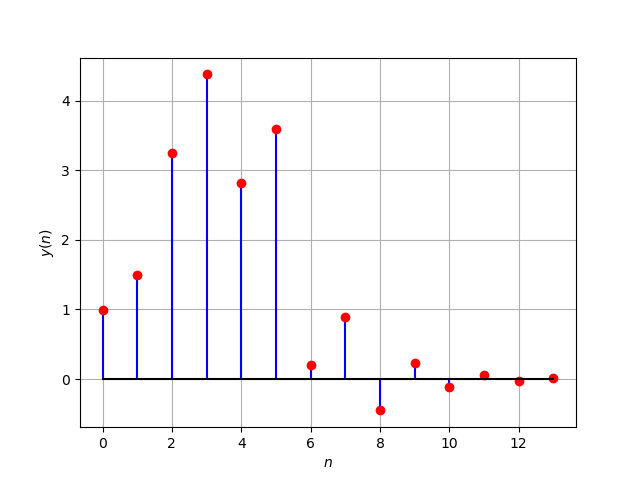
\includegraphics[width=\columnwidth]{figs/matrix.png}
\caption{$y(n)$ from DFT Matrix}
\label{fig:yn_DFT_matrix}
\end{figure}
\section{\textbf{EXERCISES}}
\noindent Answer the following questions by looking at the python code in Problem \ref{py:audio_filter}.
\begin{enumerate}[label=\thesection.\arabic*]
\item
The command
\begin{lstlisting}
	output_signal = signal.lfilter(b, a, input_signal)
	\end{lstlisting}
in Problem \ref{py:audio_filter} is executed through the following difference equation
\begin{equation}
\label{eq:iir_filter_gen}
 \sum _{m=0}^{M}a\brak{m}y\brak{n-m}=\sum _{k=0}^{N}b\brak{k}x\brak{n-k} 
\end{equation}
%
where the input signal is $x(n)$ and the output signal is $y(n)$ with initial values all 0. Replace
\textbf{signal. filtfilt} with your own routine and verify.\\

\solution Below code plots the input signal:

\begin{lstlisting}
https://github.com/Avyaaz13/Audio-Filtering/blob/main/Audio%20Filtering/codes/6.1_filtfilt.py
\end{lstlisting}
\begin{figure}[!ht]
\centering
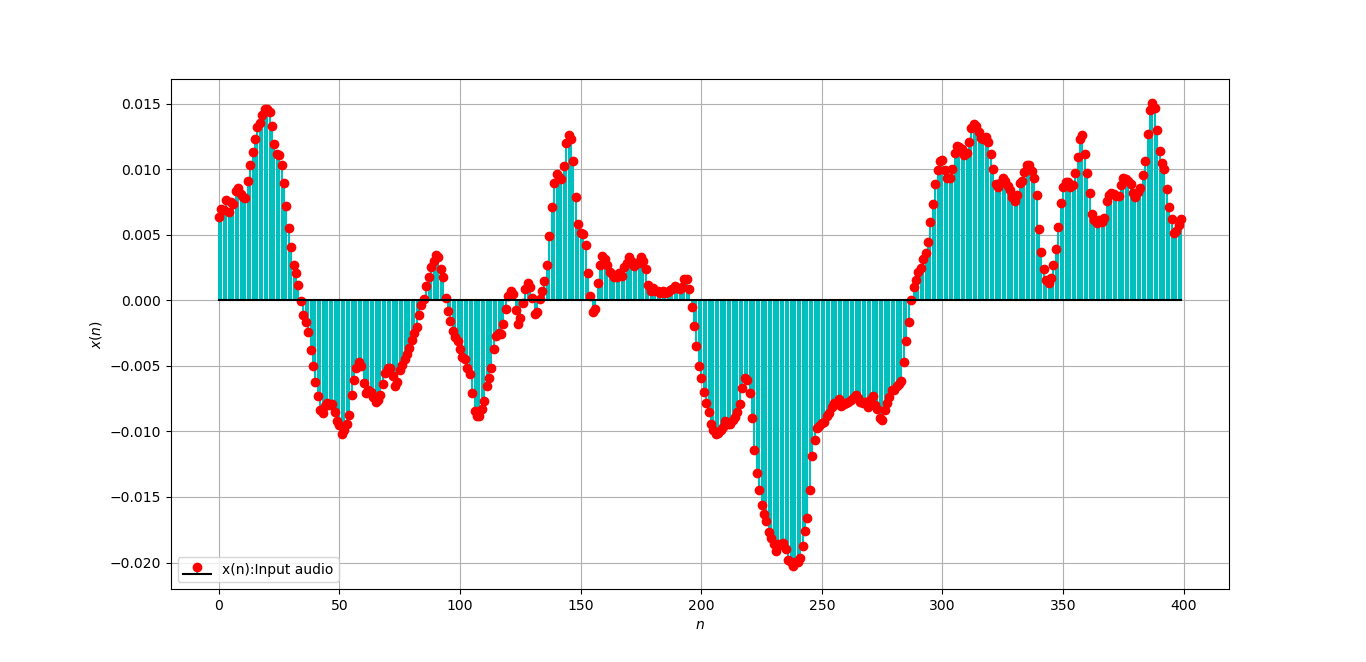
\includegraphics[width=1.2\columnwidth]{figs/xn_custom.png}
\caption{$x(n)$ vs $n$}
\label{fig:x(n) vs n}
\end{figure}
The below code gives the output of an Audio Filter without using the built in function signal.filtfilt.
\begin{figure}[!ht]
\centering
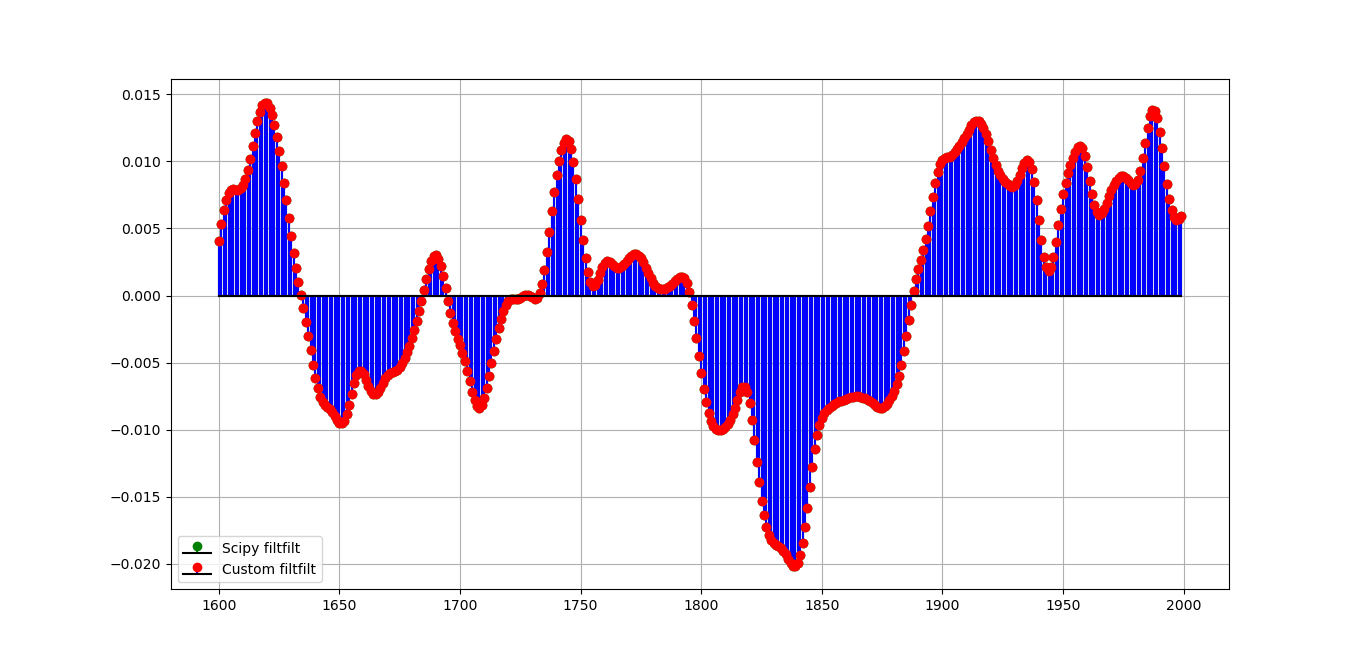
\includegraphics[width=1.2\columnwidth]{figs/Figure_1.png}
\caption{Verifying the output using and without using {\em signal.filtfilt}}
\label{fig:6.1}
\end{figure}

The below code gives the output of an Audio Filter without using the built in function signal.lfilter.
\begin{lstlisting}
https://github.com/Avyaaz13/Audio-Filtering/blob/main/Audio%20Filtering/codes/lfilt.py
\end{lstlisting}
\begin{figure}[!ht]
\centering
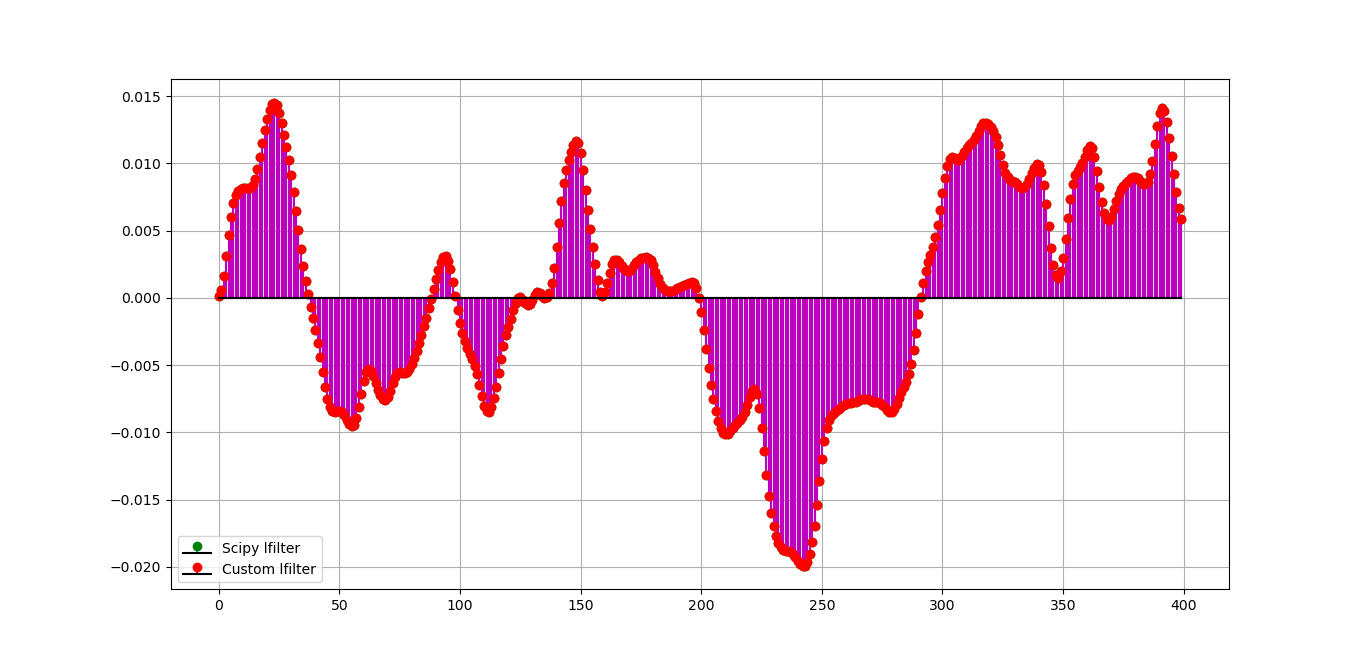
\includegraphics[width=1.2\columnwidth]{figs/lfilt.png}
\caption{Verifying the output using and without using {\em signal.lfilter}}
\label{fig:6.1_lfilt}
\end{figure}


\item Repeat all the exercises in the previous sections for the above $a$ and $b$.\\
\solution The code in \ref{py:audio_filter} generates the values of $a$ and $b$  which can be used to generate a difference equation.
\begin{align}
a &= \begin{bmatrix}
1 & -1.87302725 & 1.30032695 & -0.31450204 
\end{bmatrix}\nonumber\\
b &= \begin{bmatrix}
0.0140997 & 0.0422991 & 0.0422991 & 0.0140997 
\end{bmatrix}\nonumber
\end{align}
And,
\begin{align}
    M &= 3\\
    N &= 3
\end{align}
From \ref{eq:iir_filter_gen} 
\begin{align}
    &a\brak{0}y\brak{n} + a\brak{1}y\brak{n-1}+a\brak{2}y\brak{n-2}+a\brak{3}\notag\\ \notag &y\brak{n-3} =   b\brak{0}x\brak{n} + b\brak{1}x\brak{n-1}\\ \notag &+b\brak{2}x\brak{n-2}+b\brak{3}x\brak{n-3} 
\end{align}

Difference Equation is given by :
\begin{multline}
      y(n) - 1.87 y(n - 1) + 1.3 y(n - 2) - 0.31 y(n - 3) \nonumber \\
	= 0.014 x(n) + 0.042 x(n - 1) + 0.042 x(n - 2) \\\nonumber
        + 0.014 x(n - 3) 
\end{multline}

From \eqref{eq:iir_filter_gen} 
\begin{align}
    H(z) &= \frac{b(0) + b(1) z^{-1} + b(2) z^{-2} + \ldots + b(N) z^{-N}}{a(0) + a(1) z^{-1} + a(2) z^{-2} + \ldots + a(M) z^{-M}}\\
    H(z) &= \frac{\sum_{k = 0}^{N}b(k)z^{-k}}{\sum_{k = 0}^{M}a(k)z^{-k}} \label{eq:trans-func}
\end{align}

Below code plots\figref{fig:H(w)} Frequency response:
\begin{lstlisting}
https://github.com/Avyaaz13/Audio-Filtering/blob/main/Audio%20Filtering/codes/6.2_Hz_custom.py
\end{lstlisting}
\begin{figure}[!ht]
\centering
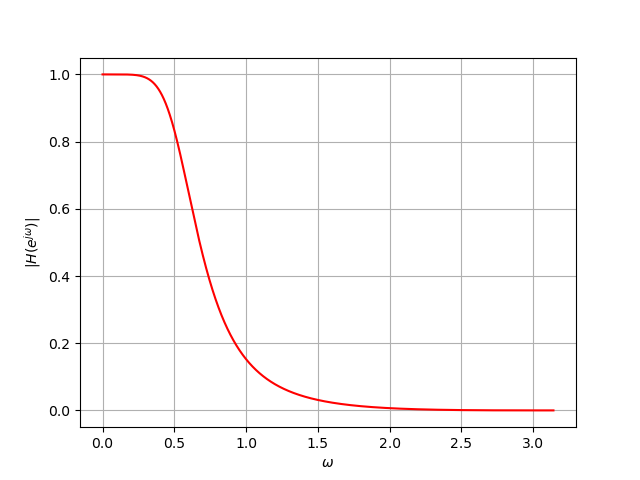
\includegraphics[width=\columnwidth]{figs/Filter_Response.png}
\caption{Frequency Response of Audio Filter}
\label{fig:H(w)}
\end{figure}

Below code plots \figref{fig: zero-pole} Zero-Pole graph:
\begin{lstlisting}
https://github.com/Avyaaz13/Audio-Filtering/blob/main/Audio%20Filtering/codes/zero-pole.py
\end{lstlisting}
\begin{figure}[!ht]
\centering
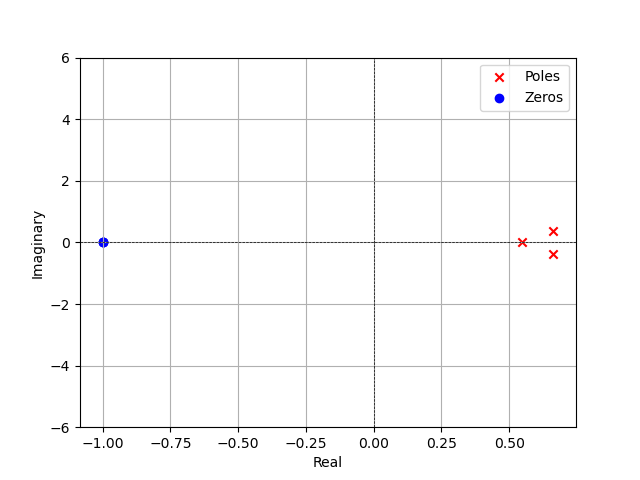
\includegraphics[width=\columnwidth]{figs/pole_zero.png}
\caption{Zero-Pole plot}
\label{fig: zero-pole}
\end{figure}

\begin{align}
\because&\text{Zeroes}\approx \begin{bmatrix}
-1 & -1 & -1
\end{bmatrix}\nonumber\\
&\text{Poles}= \begin{bmatrix}
0.663 + 0.368j & 0.663 - 0.368j & 0.547 
\end{bmatrix}\nonumber
\end{align}

Now,
\begin{align}
    \delta\brak{n-k} \system{Z} z^{-k}\label{eq:res-1}
\end{align}
Let us assume that a causal sequence is to be obtained using \textbf{Long Division Method:}
\begin{multline}
H(z) = 0.014 \,+\, 0.069z^{-1}\, +\, 0.153z^{-2} \\ + \,0.215z^{-3} \,+ \, 0.226z^{-4} \,+\, 0.192z^{-5} + ......
\end{multline}
Taking inverse z transform of \eqref{eq:trans-func} by using \eqref{eq:res-1}:
\begin{multline}
h(n) = 0.014\delta(n) \,+\, 0.069 \delta(n - 1)\, +\, 0.153\delta(n - 2) \\ + \,0.215\delta(n - 3) \,+ \, 0.226\delta(n - 4) \,+\, 0.192 \delta(n - 5) + ......
\end{multline}

% h(0) = 0.014099708769044324
% h(1) = 0.0687082650263731
% h(2) = 0.15265734752823878
% h(3) = 0.2151222584561684
% h(4) = 0.22603427726013037
% h(5) = 0.19165013578935938

Below is the code which plots the {\em Impulse response:}
\begin{lstlisting}
 https://github.com/Avyaaz13/Audio-Filtering/blob/main/Audio%20Filtering/codes/6.2_hn.py
 \end{lstlisting}
\begin{figure}[!ht]
\centering
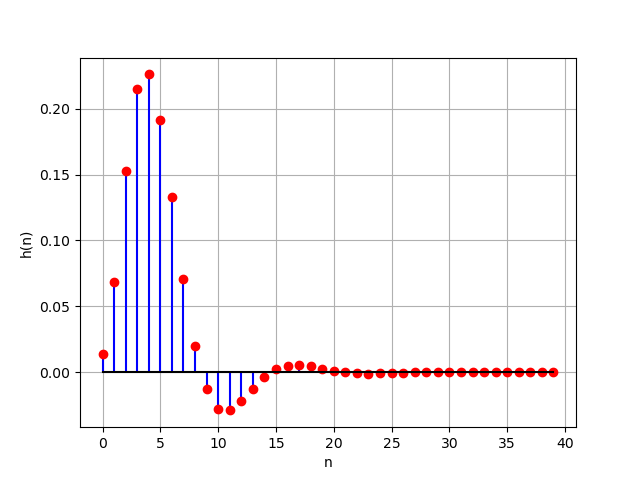
\includegraphics[width=\columnwidth]{figs/h(n)_custom.png}
\caption{$h(n)$ vs $n$}
\label{fig:hn_custom}
\end{figure}
\textbf{Stability of h(n)}:\\
According to \eqref{eq:stb_condn}
\begin{align}
H\brak{z} &= \sum_{n = 0}^{\infty} h\brak{n}z^{-n}\\
H(1)&= \sum_{n = 0}^{\infty}h(n)  = \frac{\sum_{k = 0}^{N}b(k)}{\sum_{k = 0}^{M}a(k)}< \infty
\end{align}
As both $a\brak{k}$ and $b\brak{k}$ are finite length sequences they converge.\\

\item Compute 
\begin{equation}
\label{eq:convolve}
y(n) = x(n)*h(n) = \sum_{k=-\infty}^{\infty}x(k)h(n-k)
\end{equation}

Comment. The operation in \eqref{eq:convolve} is known as
{\em convolution}.
%
\\
\solution Below code plots \figref{fig:ynconv6} 

\begin{lstlisting}
https://github.com/Avyaaz13/Audio-Filtering/blob/main/Audio%20Filtering/codes/6.3_ynconv.py
\end{lstlisting}
\begin{figure}[!ht]
\centering
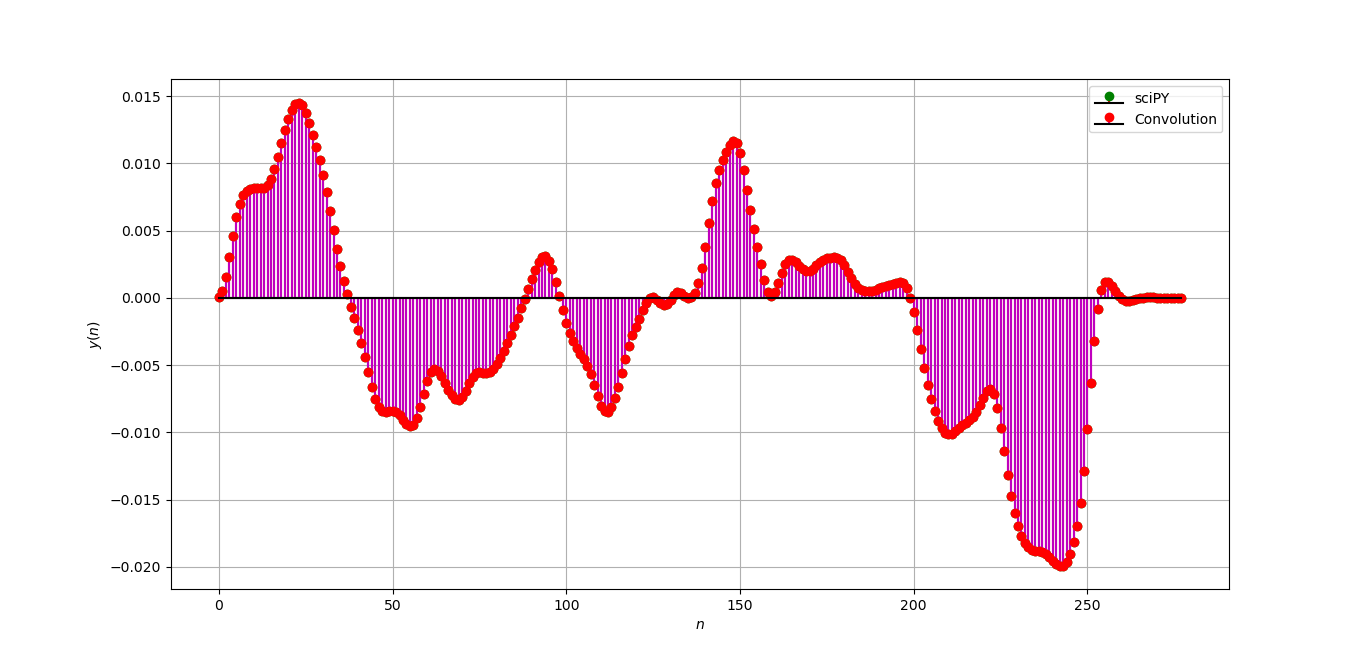
\includegraphics[width=\columnwidth]{figs/6.2_yncon.png}
\caption{$y(n)$ from the definition of convolution}
\label{fig:ynconv6}
\end{figure}

\item Compute $y(n)$ using DFT and FFT.

Below code plots \figref{fig:dft__fft} $y(n)$ using DFT and FFT:
\begin{lstlisting}
https://github.com/Avyaaz13/Audio-Filtering/blob/main/Audio%20Filtering/codes/6.4_yndft.py
\end{lstlisting}
\newpage
\begin{figure}[!ht]
\centering
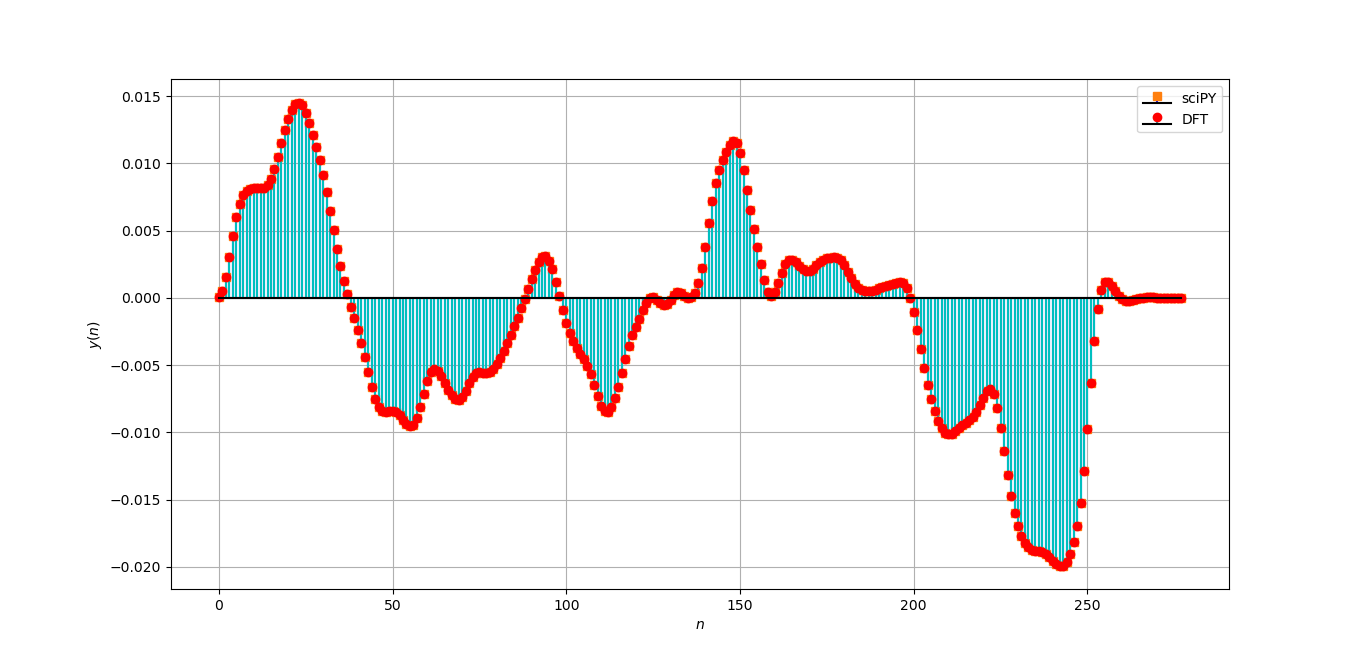
\includegraphics[width=\columnwidth]{figs/6.2_dft.png}
\caption{$y(n)$ obtained from DFT \& FFT }
\label{fig:dft__fft}
\end{figure}

\item Frequency Response of Butterworth Filter in Analog Domain:

To convert to analog domain, we can use the Bilinear Transform where we substitute:
\begin{align}
    z=\frac{1+\frac{sT}{2}}{{1-\frac{sT}{2}}}
\end{align}
Below is the code to plot Frequency Response in Analog Domain:
\begin{lstlisting}
https://github.com/Avyaaz13/Audio-Filtering/blob/main/Audio%20Filtering/codes/6_bt.py
\end{lstlisting}
\begin{figure}[!h]
    \centering
    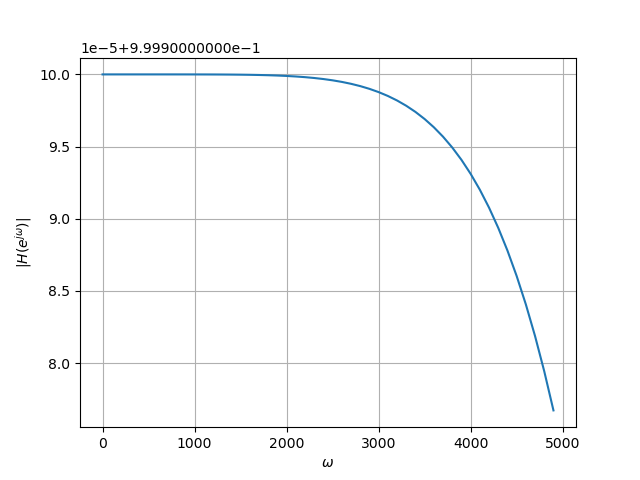
\includegraphics[width = \columnwidth]{figs/bt.png}
    \caption{Plot of Frequency Response in Analog Domain}
    \label{fig:bt}
\end{figure}
\item What is the sampling frequency of the input signal?\\
\solution The Sampling Frequency is $44.1$KHz
\item
What is type, order and  cutoff-frequency of the above butterworth filter
\\
\solution The given butterworth filter is lowpass with order = $3$ and cutoff-frequency = $4kHz$.

\item
Modify the code with different input parameters and get the best possible output.

\solution
A better filtering was found when order of the filter is 4.

\end{enumerate}


\end{document}
